%!TEX root = spack-sc15.tex

\subsection{The ARES Multi-physics Code}
\label{sec:ares}

For our final use case, we describe our experiences using Spack to build ARES.
ARES~\cite{ares1,ares2} is a 1, 2 and 3-dimensional radiation hydrodynamics code,
developed for production use at LLNL.  It can run both small, serial
and large, massively parallel jobs. ARES is used primarily in munitions modeling
and inertial confinement fusion simulations.
%
At LLNL, it runs on commodity Linux clusters and on Blue Gene/Q systems.
It also runs on the Cielo Cray XE6 system at Los Alamos National Laboratory (LANL), and
it is being ported to LANL's forthcoming Trinity Cray XC30 machine on Trinitite,
a smaller version of the full system.  The Trinity machine will consist of two partitions;
one using Intel Haswell processors and another using Intel Knights Landing processors.
Currently, only the Haswell partition is deployed on Trinitite.

\begin{figure*}[t]
	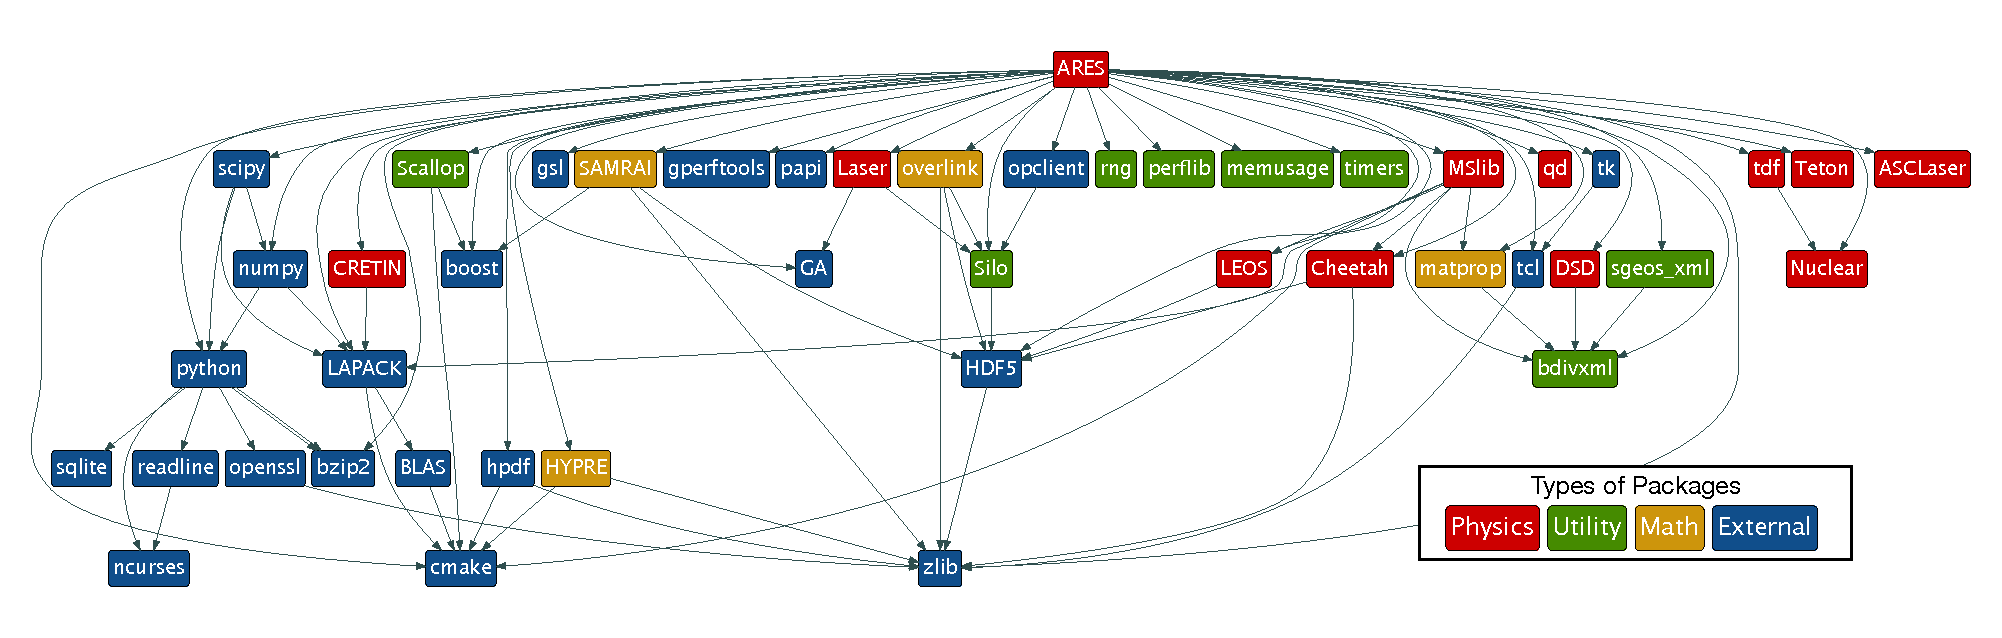
\includegraphics[width=\textwidth]{figs/ares-dot/ares-fig.pdf}
	\caption{
		Dependencies of ARES, colored by type of package.
		\label{fig:ares}
	}
\end{figure*}

ARES comprises 47 packages, with complex dependency relationships. 
Figure~\ref{fig:ares} shows the DAG for the current production configuration 
of ARES. At the top is ARES itself.  ARES depends on 11 LLNL physics packages 
(red), 4 LLNL math/meshing libraries (gold), and 8 LLNL utility libraries 
(green). The utility libraries handle tasks including logging, I/O, and 
performance measurement. ARES also uses 23 external software packages, 
including MPI, BLAS, Python, and many other libraries.  Together, these 
packages are written in a diverse set of languages including C, C++, 
Fortran, Python and tcl and uses MPI and OpenMP for parallelism.

We have configured Spack to build ARES with external MPI implementations, 
depending on the host system. This configuration exploits the vendor- 
or site-supplied MPI installation that often uses host-specific optimized 
network drivers. MPI is shown as a virtual dependency in the figure, as 
the implementation differs according to the host machine.  ARES builds its 
own Python version in order to run on machines where Python is not well 
supported, like Blue Gene/Q.  In particular, ARES builds a version of 
Python 2.7 for Blue Gene/Q, which the native software stack does not support.

Prior to using Spack, ARES managed its software stack with MixDown.
Thus, the ARES team already had some experience supporting 
automated builds of dependencies. We developed Spack packages for the LLNL 
packages in Figure~\ref{fig:ares}. Many of the external packages were already 
available in Spack, but some, such as Python, required modifications to support
the new platforms and compilers.

\newcommand{\hfmt}[1]{\textit{\scriptsize #1}}
\newcommand{\cfmt}[1]{\texttt{\scriptsize #1}}

\begin{table}\centering % mvapich2 for intel 15
\footnotesize
\begin{tabular}{|r|c|c|c|c|c|}
\hline
\multirow{2}{*}{} & \multicolumn{3}{|c|}{\hfmt{Linux}}                      & {\hfmt{BG/Q}}     & {\hfmt{Cray XE6}} \\\cline{2-6}
                  & {\hfmt{MVAPICH}} & {\hfmt{MVAPICH2}} & {\hfmt{OpenMPI}} & {\hfmt{BG/Q MPI}} & {\hfmt{Cray MPI}} \\\hline
{\hfmt{GCC}}      & {\cfmt{C P L D}} &                   &                  &                   &                   \\\hline
{\hfmt{Intel 14}} & {\cfmt{C P L D}} &                   &                  &                   &                   \\\hline
{\hfmt{Intel 15}} & {\cfmt{C P L D}} & {\cfmt{D}}        &                  &                   &                   \\\hline
{\hfmt{PGI}}      &                  & {\cfmt{D}}        & {\cfmt{C P L D}} &                   & {\cfmt{C L D}}    \\\hline
{\hfmt{Clang}}    & {\cfmt{C P L D}} &                   &                  & {\cfmt{C L D}}    &                   \\\hline
{\hfmt{XL}}       &                  &                   &                  & {\cfmt{C P L D}}  &                   \\\hline
\end{tabular}
\caption{
	Configurations of ARES built with Spack: \newline
	(C)urrent and
	(P)revious production, (L)ite, and (D)evelopment).
	\label{tab:ares-configs}
}
\end{table}

Table~\ref{tab:ares-configs} shows configurations of ARES that the ARES
team tests nightly.  The rows and columns show architectures, compilers, and MPI versions.
The ARES Spack package supports four different code configurations:
the current (C) and previous (P) production versions, a ``lite'' version (L) that includes
a smaller set of features and dependencies, and a development version (D).
Each cell in the table indicates the ARES configurations built for an architecture,
compiler, and MPI combination. Each configuration requires a slightly different
set of dependencies and dependency versions, but one common ARES package supports
all of them with conditional logic on versions and variants.

Altogether, the initial packaging effort for ARES took roughly two months,
half time, for an experienced build engineer. As shown in the table, 32
different configurations have been run using Spack
(some of 4 versions on each of 10 architecture-compiler-MPI combinations).
Prior to using Spack, only Linux/Intel configurations were automated. The ARES 
team listed a number of key features that enabled the increased automation:
\begin{enumerate}
\item Spack's version tracking and optional dependencies were required to
      build the four configurations with correct libraries;
\item The spec syntax allowed build scripts to concisely test compiler,
      compiler version, and dependency versions: a necessity
      for handling the different architectures;
\item Patching packages for particular platforms was
      necessary to build many packages; and
\item Using a DSL embedded in Python was a significant benefit;
      certain packages required custom scripting to patch.
\end{enumerate}

The ARES team also mentioned two potential long-term payoffs. First, Spack 
allows the team to test with Clang.  This compiler is not currently used in
production but probably will be on future LLNL machines. Testing with Clang 
revealed many incompatibilities, which were patched with Spack. The team is 
communicating these changes back to library developers, who will integrate 
them in future versions. In this case, build automation has allowed more 
testing, which helps both ARES and LLNL library developers build more robust 
software. Second, other LLNL code teams use many libraries that ARES uses.
The LLNL code teams have begun creating an internal repository of Spack 
build recipes.  Leveraging this repository will make packaging the next 
code significantly easier.
